% !TEX root = ../ITGO.tex

%\subsection*{Pressure vessel design problem}

In the pressure vessel design problem, the objective is to minimize the total manufacturing cost, including the cost of the material, forming and welding costs \citep{PV}. The problem is subject to three linear and one nonlinear inequality constraint, and its structure is shown in Figure \ref{fig:PV}. The four variables are the thickness of the shell ($x_1 = T_s$), the thickness of the head ($x_2 = T_h$), the inner radius ($x_3 = R$), and the length of the cylindrical section of the vessel ($x_4 = L$). This is an example of a mixed integer problem, where the first and second variables are constrained to be integers. The value of the objective function at the best known feasible solution is around $f(\bm{x}^*) = 6059.7143$. The mathematical formulation for the pressure vessel problem can be expressed as follows:

\vspace{-0.5cm}

\begin{align*}
\textbf{Minimize:} & \\
& f(\bm{x}) = 0.6224z_1x_3x_4 + 1.7781z_2x_3^2 + 3.1661z_1^2x_4 + 19.84z_1^2x_3 \\[0.5em]
\textbf{subject to:} &\\
& g_1(\bm{x}) = -z_1 + 0.193x_3 \leq 0 \\
& g_2(\bm{x}) = -z_2 + 0.00954x_3 \leq 0 \\
& g_3(\bm{x}) = -\pi x_3^2x_4^2 - \frac{4}{3} \pi x_3^3 + 1,296,000 \leq 0 \\
& g_4(\bm{x}) = x_4 - 240  \leq 0 \\[0.5em]
\textbf{where:} & \\
& z_1 = 0.0625x_1 \\
& z_2 = 0.0625x_2 \\[0.5em]
\textbf{with bounds:} & \\
& 1 \leq x_1, x_2 \leq 99, \quad 10 \leq x_2, x_3 \leq 200, \quad x_1, x_2 \in \mathbb{Z}
\end{align*}

\vspace{0.5cm}

\begin{figure}[h]
    \begin{center}
    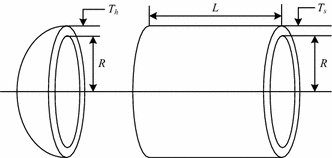
\includegraphics[scale=0.6]{img/Problems/PV.png}
    \end{center}
    \captionsetup{justification=centering}
    \caption{Schematic view of pressure vessel design problem.}\label{fig:PV}
\end{figure}
